\chapter{Operating System}

\section{Introduction}

An operating system (\textbf{OS}) is the software that manages the computer hardware, creating some logical resources that other software and users can use. It's the logical support which controls and manages the physical components.

\begin{center}
    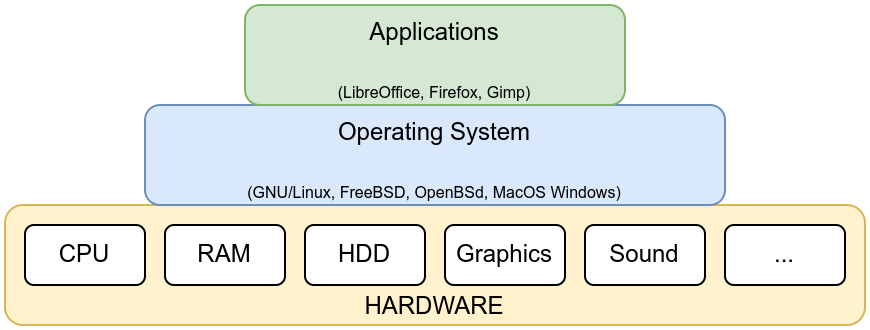
\includegraphics[width=0.9\linewidth]{operating_system.png}
\end{center}

Before the existence of operating systems, the hardware was available directly to the program, so every program must implement the access to the memory, the hard disk, how to read/write files...

\section{Software hierarchy}
The computer runs software, and this software can be classified:

\begin{itemize}
    \item \textbf{System's software}: Controls and manages the hardware of the computer. In this group: \textbf{operating systems}, \textbf{drivers} and \textbf{firmwares}.

    \item \textbf{Service programs}: Those are the networking services, system's services, and some services that the operating system uses. For example: networking management tools, disk partitioners, process manager ...

    \item \textbf{Utility programs}: The software that the end users use in order to do some basic stuff. Word processors, music utilities, games, ...
\end{itemize}

In this chapter we are going to focus on the system software, specifically the \textbf{operating system}.


\section{History of operating systems}
Let's see a brief history of operating systems.

\subsection{No operating systems (0-generation)}
The first computers were mainframes (big computers used by organizations), which didn't have any form of operating system.

The user which wanted to use the computer had to  schedule a period of time, because those computers hadn't got time sharing, only one program could run in each time.

First programs were coded in \textbf{machine code}, which is represented with '0' and '1', also called \textbf{binary code}.

Those programs had full access to the hardware, and because of that, every program had to implement access to those resources.

This period started with the digital computers until the late 1950s.

\begin{center}
    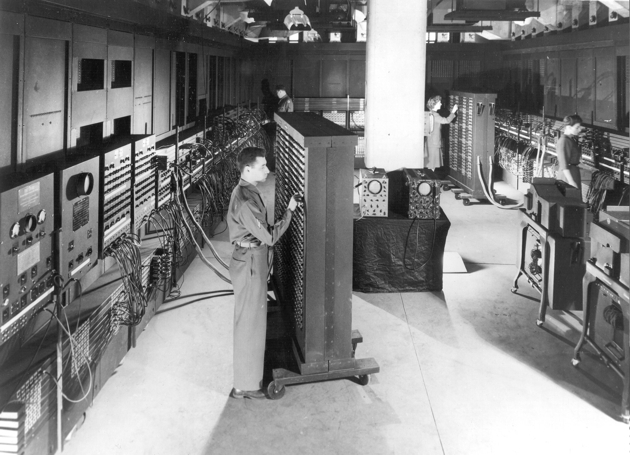
\includegraphics[width=0.6\linewidth]{ENIAC.jpg}
    \vspace{-10pt}\captionof{figure}{\href{https://en.wikipedia.org/wiki/ENIAC}{ENIAC computer. Source: Wikipedia}}\vspace{-13pt}
\end{center}


\hypertarget{1st_generation}{}
\subsection{Batch processing (1st generation)}
The computers became faster, and in order to no waste time, the \textit{\textbf{monitors}} were developed (the forerunners of operating systems). Those \textit{monitors} could process a series, or “batch”, of programs, often from magnetic tape.

\begin{center}
    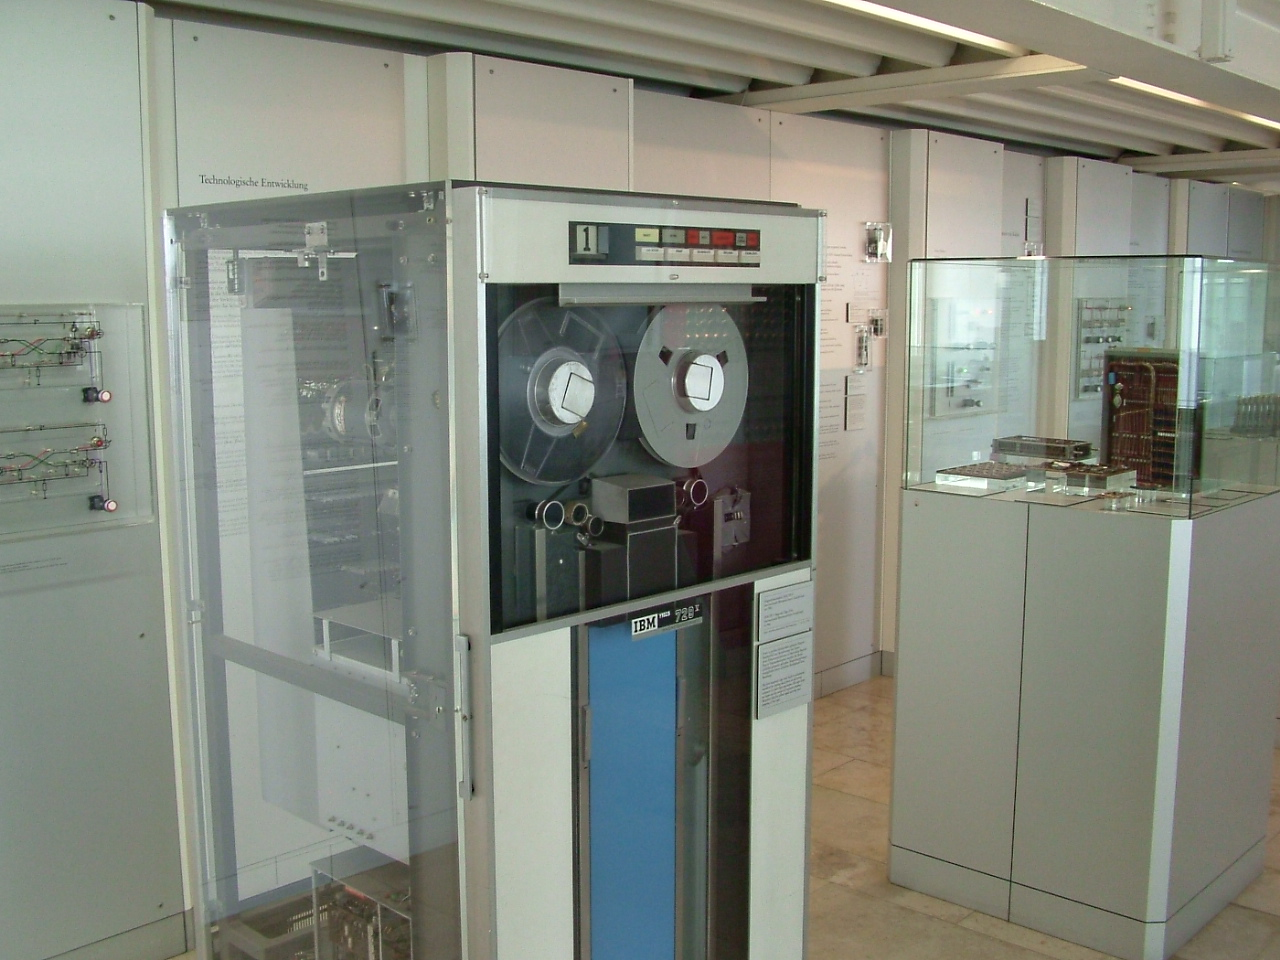
\includegraphics[width=0.6\linewidth]{tape.jpg}
    \vspace{-10pt}\captionof{figure}{\href{https://en.wikipedia.org/wiki/Magnetic-tape_data_storage}{Magnetic tape from IBM. Source: Wikipedia}}\vspace{-13pt}
\end{center}

The monitor would be loaded into the computer and run the first job of the batch. At the end of the job it would regain control and load and run the next until the batch was complete. The \textbf{output} of the batch would be written to magnetic tape or printed.


\subsection{Second generation}
In the 1960s, with the introduction ot the \href{https://en.wikipedia.org/wiki/Integrated_circuit}{integrated circuits}, the computers increased in speed, so the operating systems evolved trying to use this speed, using new techniques:

\begin{itemize}
    \item \textbf{Multiprogramming}: In any modern operating system there can be more than one instance of a program loaded in memory at the same time. For example, more than one user could be executing the same program, each user having separate copies of the program loaded into memory

    \item \textbf{Spooling}: Is a specialized form of multi-programming for the purpose of copying data between different devices. Was used to mediate access to punched card readers and punches, magnetic tape drives, and other slow, sequential I/O devices.

    \item \textbf{Buffering}:\textbf{Data buffer} (or just buffer) is a region of a memory used to temporarily store data while it is being moved from one place to another.
\end{itemize}

\subsection{Third generation}
With the evolution of computers, which began to allow the use of several processors, and more complex systems, operating systems evolved along with them. This generation is between 1965 and 1980.

\begin{itemize}
    \item \textbf{Multitasking}: Is the concurrent execution of multiple processes over a certain period of time. New tasks can interrupt already started ones before they finish, instead of waiting for them to end.

    When the computer has multiple processors, the multitasking is real, because each processor can execute one process at the same time.

    \begin{minipage}{0.6\linewidth}
        \item \textbf{Virtual memory}: Is a memory management technique that allows the use of the hard disk as part of the main memory of the system.

        The combination of real physical memory with the hard disk creates a “virtual memory” that can be used by the operating system.

        The negative part is that the hard disk is slower in reading and writing, and therefore the performance when using that part of the virtual memory is slower.
    \end{minipage}
    \hfill
    \begin{minipage}{0.3\linewidth}
        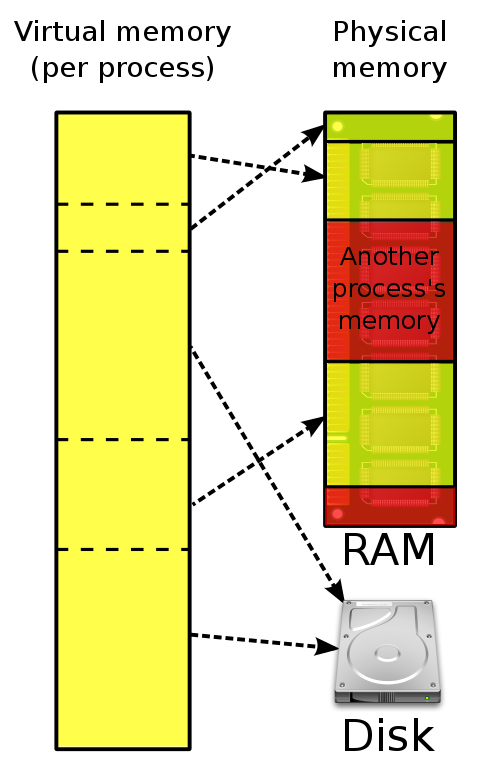
\includegraphics[width=0.9\linewidth]{virtual_memory.png}
        \vspace{-10pt}
        \captionof{figure}{\href{https://en.wikipedia.org/wiki/Virtual_memory}{Virtual Memory. Source: Wikipedia}}
    \end{minipage}

    \vspace{10pt}
    \item \textbf{Expert systems}: Specialized operating systems are created for certain tasks for specific systems. For example, \textbf{real-time systems}, which are specialized systems where the answers have to be given in a maximum time to ensure its correct operation.
\end{itemize}

\subsection{Fourth generation}
The fourth generation of the operating system took place around 1980 and is being used till now. This generation goes hand in hand with personal computers, which already have processors that contain thousands of transistors and are starting to get cheaper.

\begin{itemize}

    \item \textbf{Local Area Network (LAN)}: At the beginning of the 1980s, the first commercial networks for the transfer of information began to be created, so the operating systems must allow the use of these networks. Thanks to this, today we can browse the Internet as we do and we can send and receive information from other computers.

    \begin{minipage}{0.6\linewidth}
        \item \textbf{Distributed computing}: Distributed systems are groups of networked computers which share a common goal for their work.

        In distributed computing, each processor has its own private memory (distributed memory). Information is exchanged by passing messages between the processors. Each computer has its own local memory, and information can be exchanged only by passing messages from one node to another by using the available communication links
    \end{minipage}
    \hfill
    \begin{minipage}{0.34\linewidth}
        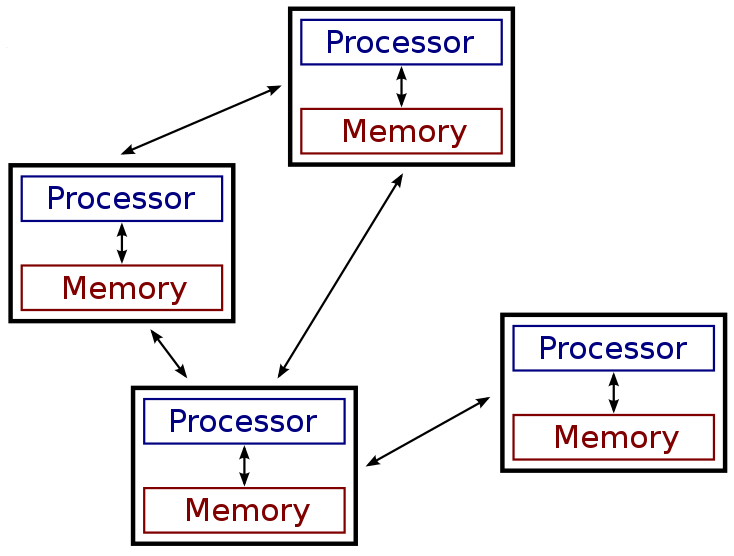
\includegraphics[width=0.9\linewidth]{distributed.png}
        \vspace{-10pt}
        \captionof{figure}{\href{https://en.wikipedia.org/wiki/Distributed_computing\#Parallel_and_distributed_computing}{Source: Wikipedia}}
    \end{minipage}
\end{itemize}



\section{Components}

Each operating system is different, but we can say that the basic components are the same for all of them. The most important components that we are going to study are the following:

\begin{center}
    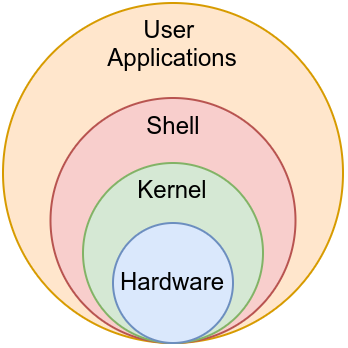
\includegraphics[width=0.4\linewidth]{jerarquia.png}
    \vspace{-10pt}
    \captionof{figure}{Operating System's componentes}
\end{center}



\subsection{Kernel}
The kernel is the central part of the operating system and is responsible for carrying out all the secure communication between the rest of the software and the hardware of the computer.

\vspace{-10pt}
\begin{center}
    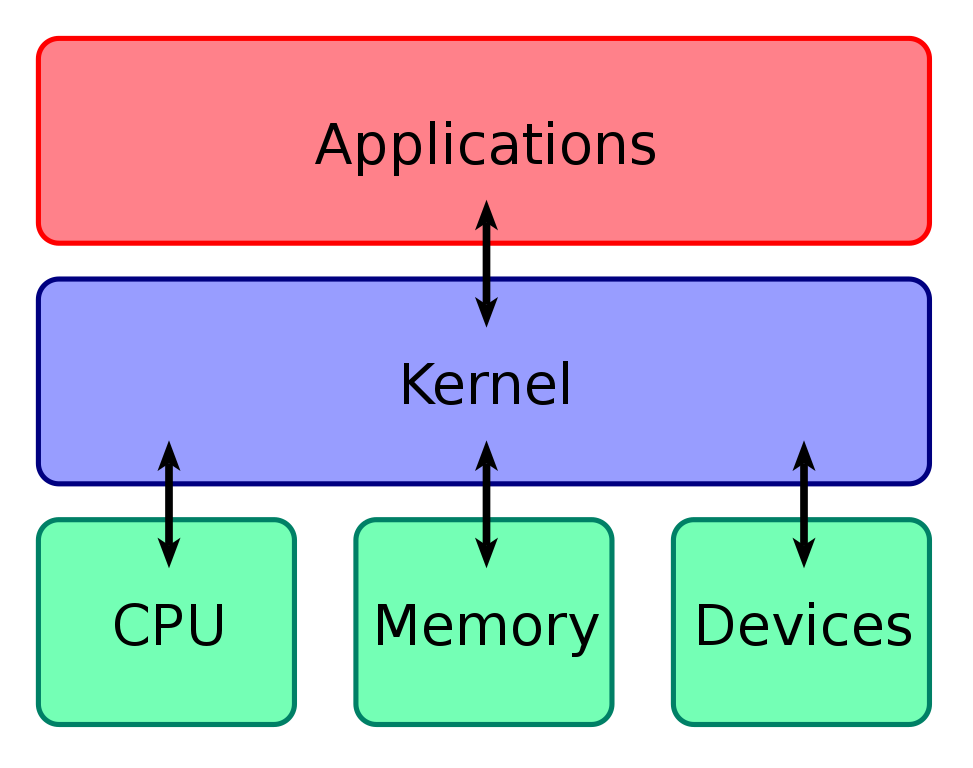
\includegraphics[width=0.5\linewidth]{kernel.png}
    \vspace{-10pt}
    \captionof{figure}{\href{https://en.wikipedia.org/wiki/File:Kernel_Layout.svg}{The kernel connects the applications to the hardware. Source: Wikipedia}}
\end{center}


On most systems, the kernel is one of the first programs loaded on startup (after the bootloader). It handles the rest of startup as well as the CPU,  memory, peripherals, and input/output (I/O).


\subsubsection{Design}

There are different kernel architecture designs.

\begin{itemize}
    \item \textbf{Monolithic kernel}: The first structure used by operating systems was the monolithic one, where is used a single-process kernel. The operating system could only execute one task at a time, composed of a set of interlocking routines in such a way that each one can call any other.

    This is the traditional design of \href{https://en.wikipedia.org/wiki/Unix}{\textbf{Unix}} systems. A monolithic kernel is one single program that contains all of the code necessary to perform every kernel-related task.

    The \textbf{\href{https://en.wikipedia.org/wiki/Linux_kernel}{Linux}} kernel is one of the most representative of this design.

    \item \textbf{Micro-kernels}: Describes an approach to operating system design by which the functionality of the system is moved out of the traditional "kernel", into a set of "servers" that communicate through a "minimal" kernel.

    Most micro-kernels use a message passing system to handle requests from one server to another. They are part of the operating systems like \href{https://en.wikipedia.org/wiki/GNU_Hurd}{\textbf{GNU Hurd}} and \href{https://en.wikipedia.org/wiki/Minix}{\textbf{MINIX}}.

    \item \textbf{Hybrid (or modular) kernels}: hey are similar to micro kernels, except they include some additional code in kernel-space to increase performance. These kernels represent a compromise that was implemented by some developers to accommodate the major advantages of both monolithic and micro kernels.

    Hybrid kernels are used in most commercial operating systems, such as Microsoft Windows 10 and Apple's own macOS.

    \item \textbf{In layers or levels}: The design of these operating systems is built on top of the hardware in virtual overlapping levels until reaching the end user level. Designed for \href{https://en.wikipedia.org/wiki/THE_multiprogramming_system}{THE operating system} in 1968 by E. W. Dijkstra's team.
    \begin{itemize}
        \item \textbf{Level 0}: The hardware.
        \item \textbf{Level 1}: The CPU management.
        \item \textbf{Level 2}: The memory management, which allow to allocate memory to processes.
        \item \textbf{Level 3}: Dealt with communication between the operating system and the system console..
        \item \textbf{Level 4}: Managed all I/O between the devices attached to the computer.
        \item \textbf{Level 5}: Consisted of user programs.
    \end{itemize}


    \begin{center}
        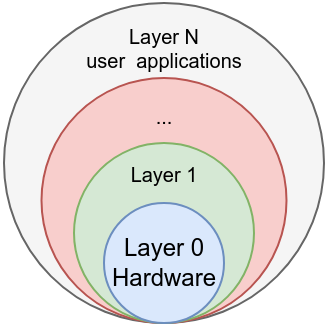
\includegraphics[width=0.5\linewidth]{layered.png}
    \end{center}
\end{itemize}

An operating system is a very complex program, so even if its main design is one of those previously mentioned, it is most likely that it will also make use of other designs as far as possible.

For example, Linux is a monolithic kernel, but it also has the option to load/unload drivers (it's modular too).


\subsection{Shell}
The “\textbf{shell}”, in operating systems, is the computer program that exposes an operating system's services to a human user or other programs.

In general, operating system shells use either a command-line interface (\textbf{CLI}) or graphical user interface (\textbf{GUI}).



\begin{mycode}{\textbf{BASH} command line interface (CLI) in GNU/Linux}{console}{}
ruben@vega:/etc/etckeeper $ ls -lh

total 48K
drwxr-xr-x 2 root root 4,0K abr 13 09:36 commit.d
-rwxr-xr-x 1 root root  551 oct 28  2019 daily
-rw-r--r-- 1 root root 1,5K oct 28  2019 etckeeper.conf
drwxr-xr-x 2 root root 4,0K abr 13 09:36 init.d
drwxr-xr-x 2 root root 4,0K abr 13 09:36 list-installed.d
drwxr-xr-x 2 root root 4,0K abr 13 09:36 post-install.d
drwxr-xr-x 2 root root 4,0K abr 13 09:36 pre-commit.d
drwxr-xr-x 2 root root 4,0K abr 13 09:36 pre-install.d
drwxr-xr-x 2 root root 4,0K abr 13 09:36 unclean.d
drwxr-xr-x 2 root root 4,0K abr 13 09:36 uninit.d
drwxr-xr-x 2 root root 4,0K abr 13 09:36 update-ignore.d
drwxr-xr-x 2 root root 4,0K abr 13 09:36 vcs.d

\end{mycode}


\section{Operating system's functions}
The main function of the operating system is to manage the hardware resources of the computer and allow the execution of user programs. To do this, it must perform various functions.

\begin{itemize}
    \item \hyperlink{process_management}{Process management}
    \item RAM memory management
    \item Input/Output management
    \item File management
    \item Networking
    \item Security
\end{itemize}

We will see each of these functionalities in the following chapters.


\section{How operating systems works}

In a simplified way, an operating system works as follows:

\begin{center}
    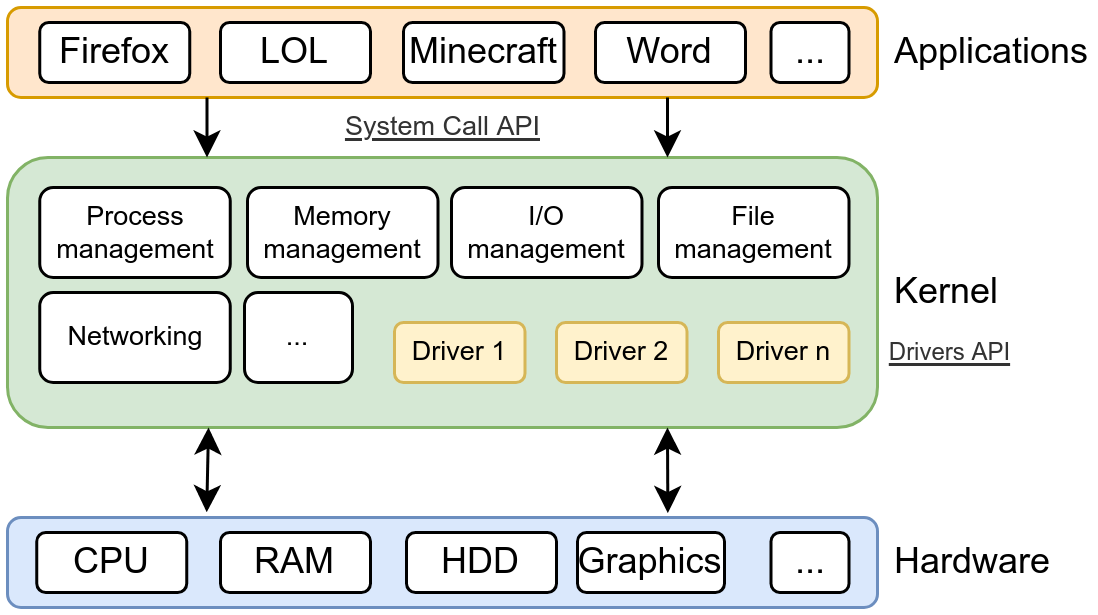
\includegraphics[width=0.75\linewidth]{how_works.png}
\end{center}



\section{Types}
Operating systems, in general, can be differentiated taking into account different points of view. We are

\subsection{Based on the number of concurrent users}
\begin{itemize}
    \item \textbf{Single user}: Only one user can execute processes in the computer each time. All hardware resources will be available to the user. For example: MS-DOS, Classic Mac OS (2001 and before), Windows 95, Windows 98.

    \item \textbf{Multi user}: Different users can execute different processes on the same microprocessor, and compete for hardware resources. For example: Linux, Mac OS X (now MacOS)
\end{itemize}

\subsection{Depending on the number of simultaneous processes}

\begin{itemize}
    \item \textbf{Monoprogramming}: Only one process can run at a time, and to run the next one, the previous one has to be finished. \hyperlink{1st_generation operating systems}{}

    \item \textbf{Multiprogramming}: Pueden ejecutar varios procesos de manera simultánea, compitiendo por el tiempo de CPU y los recursos existentes. Most current operating systems.
\end{itemize}


\subsection{Depending on system functionality}

\begin{itemize}
    \item \textbf{Workstation}: Manages a computer intended for one or more users. Connected to a network to perform tasks of a personal or professional nature. For example: Windows 7/8/10/11, Linux, MacOS.

    \item \textbf{Server}: A server is a computer that offers one or more services to other applications or users. For example: GNU/Linux, Windows Server 2012/2016/2019/2022, FreeBSD.

    \item \textbf{Distributed}: A distributed operating system manages a group of different computers and makes them appear as a single computer. Tasks are distributed among all of them to use all available resources. It is used for example in mathematical calculations, in medicine to find proteins, simulations, ...

    \item \textbf{Embedded}: They are systems that use very specific hardware. They may be limited in their functionalities, or they only allow certain tasks to be carried out or the use of certain programs (restricting the installation of some). For example: Router's operating system, \href{https://en.wikipedia.org/wiki/OpenWrt}{OpenWRT}, \href{https://en.wikipedia.org/wiki/Symbian}{Symbian}, Android*, iOS*.
\end{itemize}



\subsection{Depending on the license}
\begin{itemize}
    \item \textbf{Free Software / Software Libre}: Distributed under terms that allow users to run the software for any purpose as well as to study, change, and distribute it and any adapted versions. For example: GNU/Linux, FreeBSD, OpenBSD, GNU/Hurd, Android (some parts are free software).

    \begin{center}
        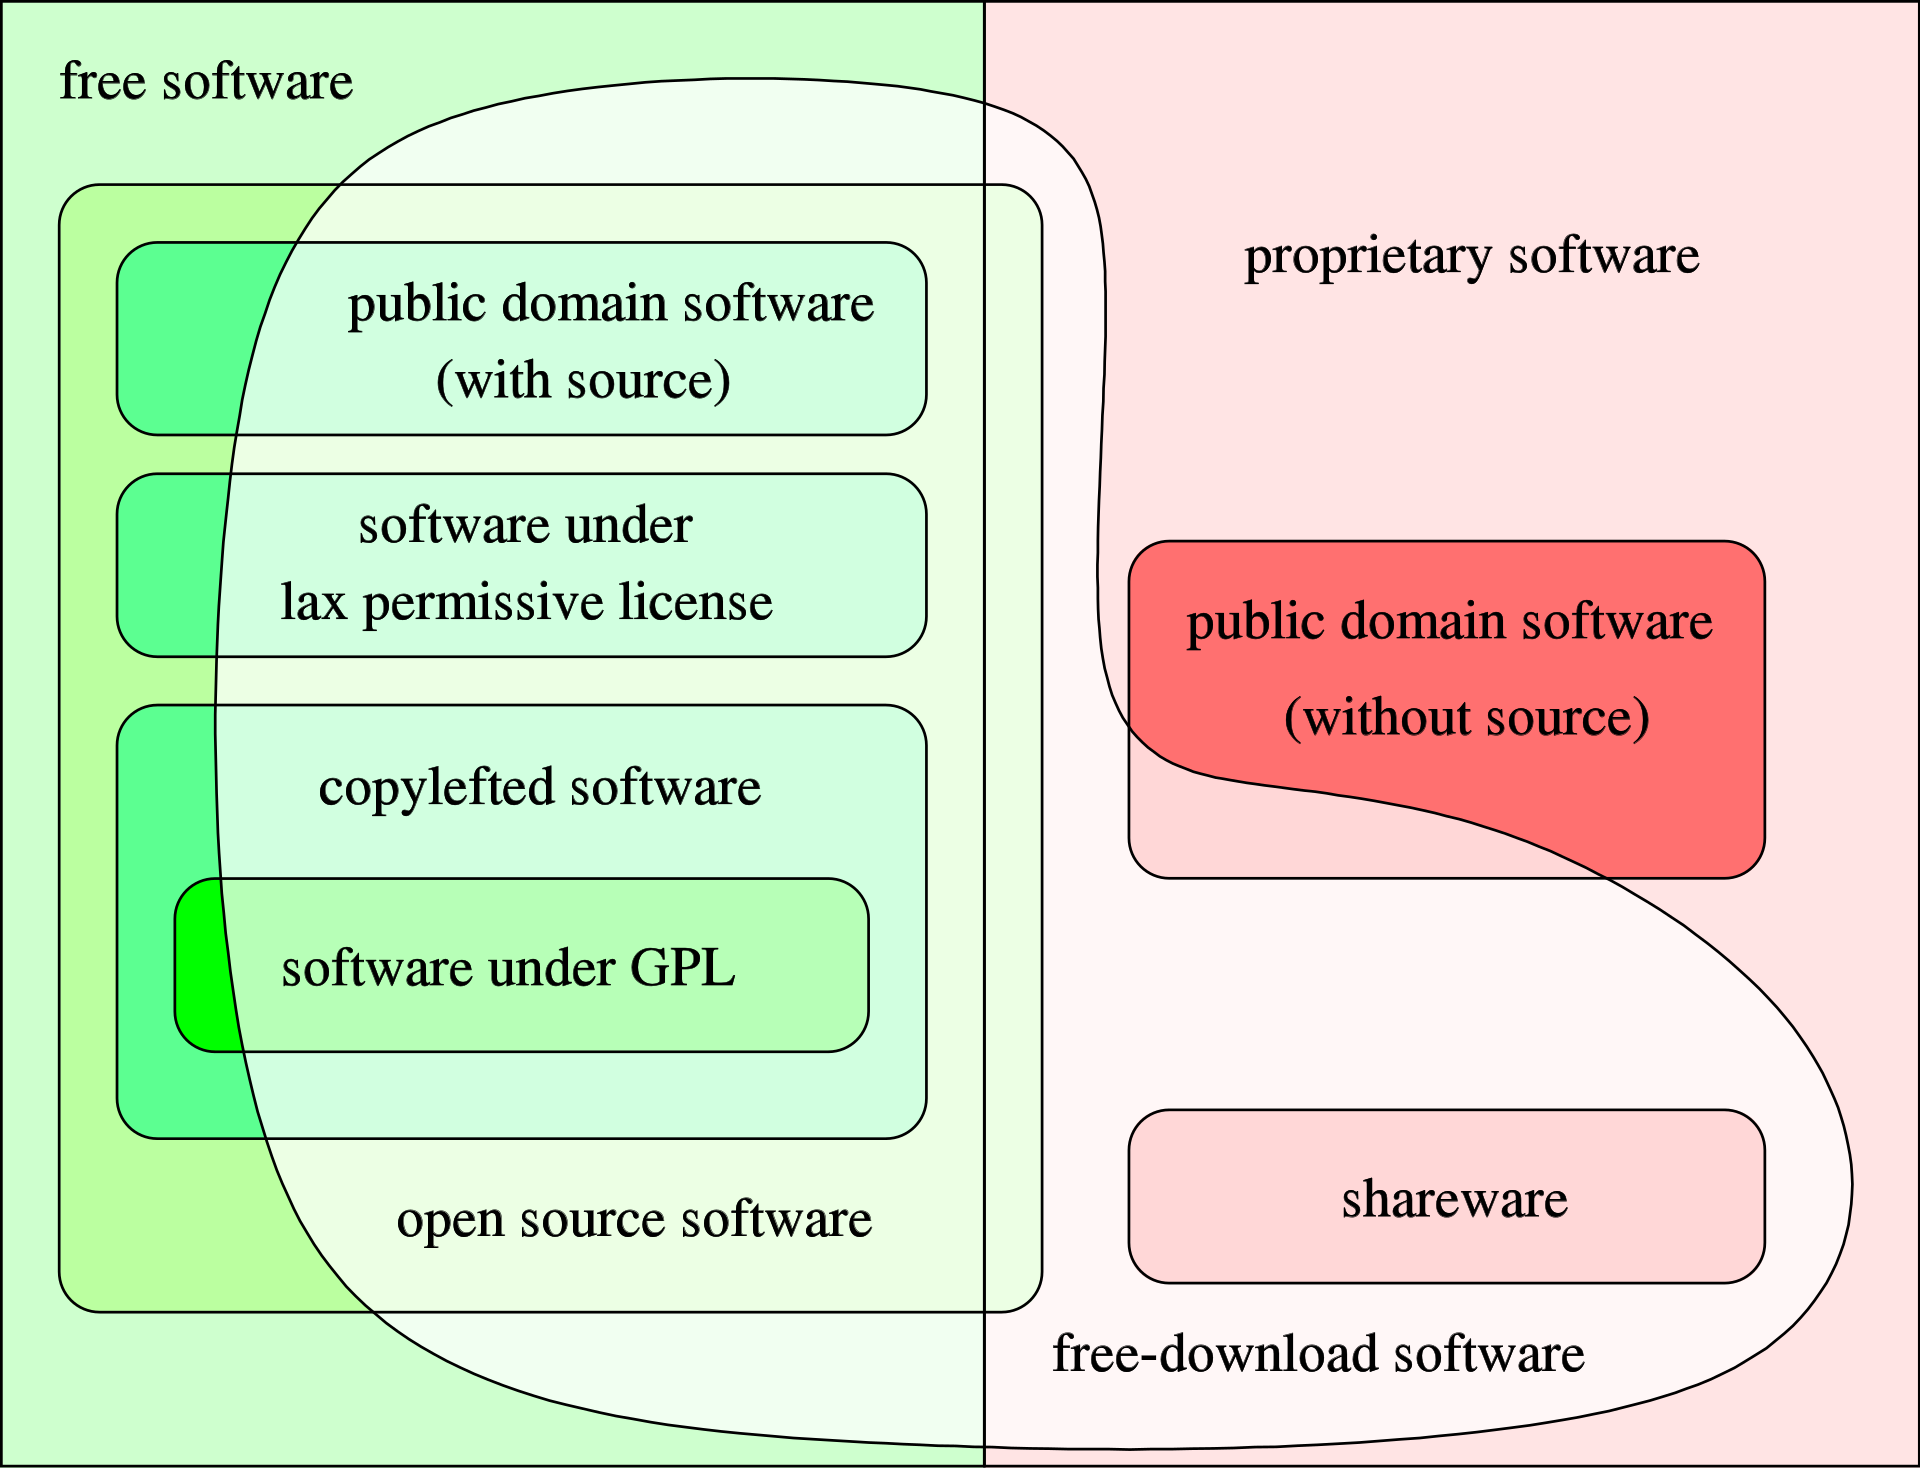
\includegraphics[width=0.65\linewidth]{free_and_nonfree_software.png}\vspace{-10pt}
        \captionof{figure}{\href{https://en.wikipedia.org/wiki/Free_software\#Definition_and_the_Four_Essential_Freedoms_of_Free_Software}{Diagram of free and nonfree software. Source: Wikipedia}}
    \end{center}

    \item \textbf{Proprietary Software}: It's the opposite of Free Software. The software creator allows you to use it under some licensing rights. For example: Windows, MacOS (the kernel is free software), iOS.
\end{itemize}



\subsection{Depending on the type of use}
\begin{itemize}
    \item \textbf{General purpose}: They can be used to perform generalized tasks. Commonly used operating systems fall into this category.

    \item \textbf{Specific purpose}: Built specifically to perform a specific task. They are usually developed as one more component within a project. For example: satellites, cars...
\end{itemize}


\hypertarget{process_management}{}
\chapter{Process management}
\textbf{A process is a program in execution}. The OS must allocate resources to processes, enable processes to share and exchange information, protect the resources of each process from other processes and enable synchronization among processes.

Processes are managed by the operating system and are made up of by:

\begin{itemize}
    \item The \textbf{instructions} of a program intended to be executed by the microprocessor. The instructions are generated with a \textbf{programming language} that will later be translated (by a compiler or an interpreter) into \textbf{machine language} (binary code that can be executed by the processor).

    \item Its \textbf{execution status} at a given moment, that is, the values of the registers of the central processing unit (CPU) for each program.

    \item The \textbf{working memory}, that is, the memory the program needs  and its contents.

    \item Other information that allows the operating system to plan.
\end{itemize}

\section{Process and threads}
In most cases \textbf{a thread is a component of a process}. The multiple threads of a given process may be executed concurrently (via multithreading capabilities), sharing resources such as memory, while different processes do not share these resources.

\infobox{\textbf{In most cases a thread is a component of a process}}

\section{Process life}

The life of a process can be summarized in the following graph:

\begin{center}
    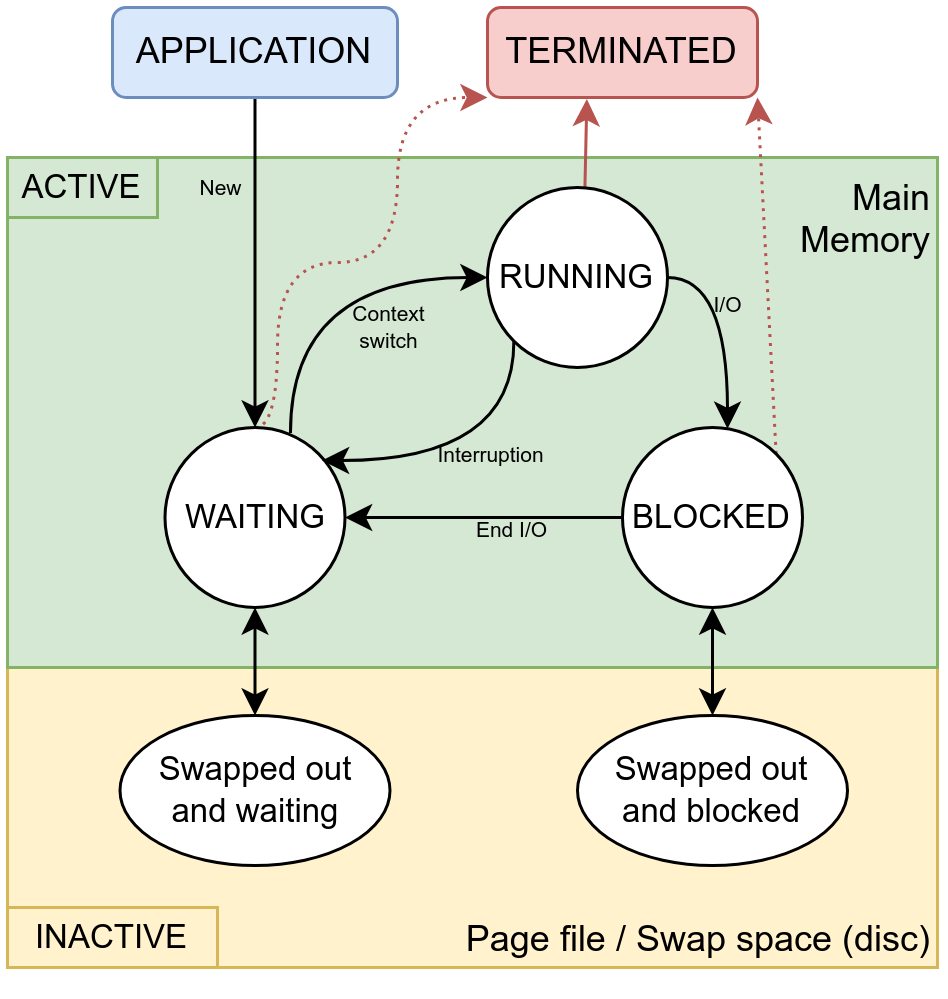
\includegraphics[width=0.65\linewidth]{process_life.png}
\end{center}

\subsection{Process status}
The processes have several states during their life, but we can separate them into two large groups:

\begin{itemize}
    \item \textbf{Active}: Competes for the processor or is in a position to do so.

    \item \textbf{Inactive}: State in which the processes that cannot compete for the processor.
\end{itemize}


\subsection{Process' states}
A process goes through different states throughout its life:

\begin{itemize}
    \item \textbf{New}: Processes in this state are loaded into memory, but are not using CPU resources. Once the process is admitted, it goes to the \textbf{waiting} state.

    \item \textbf{Waiting}: These are processes that are loaded and ready to go into the \textbf{running} state. Processes in this state are waiting for their processor turn, which is determined by the \textbf{process scheduler}.

    \item \textbf{Running}: When the process uses the resources of the processor.

    \item \textbf{Blocked}: If a process in the "running" state needs to wait for a resource (wait for \textbf{user input} or \textbf{file to open}, for example), it is assigned the "\textbf{blocked}" state. The process state is changed back to "waiting" when the process no longer needs to wait (in a blocked state).

    \item \textbf{Terminated}: Once the process finishes execution, or is terminated by the operating system, it is no longer needed. The process is removed instantly or is moved to the “terminated” state. When removed, it just waits to be removed from main memory.
\end{itemize}


There are two “special” states, which make processes considered “inactive”:

\begin{itemize}
    \item \textbf{Swapped out and waiting}.
    \item \textbf{Swapped out and blocked}.
\end{itemize}

To “swap out” means that regions of a process's memory may be really on disk and not in main memory. This is a transparent move from memory into a virtual memory system allocated on disk.


\subsection{State transitions}

A process can go from one state to another, as we have seen in the previous image. It is important to know what kind of transitions exist and the cause of those transitions.

\begin{itemize}

    %TODO: meter  “En espera: se inserta en la cola de preparados.” ??

    \item To \textbf{waiting} state:
    \begin{itemize}
        \item An application/program is \textbf{executed}.

        \item \textbf{Interruption}: If an interrupt occurs that forces the process to wait. It can happen because of the \textbf{Quantum completion}. The “quantum” of a process is equivalent to a fixed number of clock pulses or cycles. When a clock interrupt occurs that coincides with the completion of the quantum, control of the CPU is handed over to the process selected by the scheduler.

        \item \textbf{End of an I/O operation}.

        \item \textbf{Activation}. A suspended process is activated and it's queued into “waiting” queue.
    \end{itemize}

    \item To \textbf{running} state: the first process in the queue passes
    to be in “running” state when the clock has interrupted the one that was running.

    \item To \textbf{blocked} state: a process that is running and passes to
    perform an I/O operation goes to the “blocked” queue.
\end{itemize}

As with states, there are transitions to “inactive”, which occur when main memory is needed.

\section{Process control block}

A process control block (PCB) is a data structure used by computer operating systems to store all the information about a process. It is also known as a process descriptor. When a process is created, the operating system creates a corresponding process control block.

This specifies the process state i.e. new, ready, running, waiting or terminated, through the life of the process.

\errorbox{PCB must be kept in an area of memory protected from normal process access. }


\section{Process scheduling}

The OS software in charge of allocating the resources of a system among the processes that request them is called a \textbf{scheduler}.

\infobox{\textbf{The scheduler must decide which of the processes competing for possession of a given resource will receive it}}

\subsection{Strategies}
The operating system may have different strategies in terms of process scheduling:

\begin{itemize}
    \item \textbf{Appropriative strategy}: The operating system can interrupt the “running” process at any time, passing it to “waiting”, in order to give the turn to another process according to the scheduling algorithm.

    \item \textbf{Non-Appropriative strategy}: The operating system \textbf{cannot give the turn to another process unless} the one that is running terminates or is blocked by an input/output operation or by request of some other service or if it is the process itself that gives up the processor to another.
\end{itemize}

\subsection{Objectives}

Process scheduler has the following main objectives when it comes to assigning priorities:

\begin{itemize}
    \item \textbf{Equity}: All processes must be attended.

    \item \textbf{Efficiency}: The processor must be busy 100\% of the time.

    \item \textbf{Minimize wait time}: time from work becoming ready until the first point it begins execution.

    \item \textbf{minimizing latency or response time}: time from work becoming ready until it is finished in case of batch activity, or until the system responds to the user in case of interactive activity.

    \item \textbf{Maximizing fairness}: Equal CPU time to each process, or more generally appropriate times according to the priority and workload of each process.
\end{itemize}


\subsection{Scheduling algorithm}

There are different scheduling algorithms used for distributing resources among parties which simultaneously and asynchronously request them.

Those algorithms are used in routers (to handle packet traffic) as well as in operating systems (to share CPU time among both threads and processes), disk drives (I/O scheduling), printers (print spooler), most embedded systems, etc.

There are some previous concepts that we must understand before starting to see the different algorithms:
\begin{itemize}
    \item \textbf{Loading time}: Moment at which a process is loaded by the O.S. (list of waiting processes) (\textbf{L}).

    \item \textbf{CPU Utilization}: Time that keeps the CPU busy. The longer the occupation time, the better (\textbf{p}).

    \item \textbf{Exit time}: moment in which a process finishes all its execution and is removed from the system (\textbf{E}).

    \item \textbf{Waiting time} (\textbf{W}).
\end{itemize}

With all this, we can calculate the following:

\begin{itemize}
    \item \textbf{Execution time}: It is the amount of time that any process needs to execute (\textbf{t})
    \begin{center}
        $t = L + p + I/O$
    \end{center}

    \item \textbf{Service time}: The amount of time that takes a
    process to run and exit the system. The less time better.(\textbf{T})

    \begin{center}
        $T = t + W$

        $T = t_{f} - t_{i}$
    \end{center}

    \item \textbf{Service Index}: Value that represents the percentage of
    time the process is running, relative to the time it remains in the system (\textbf{I})

    \begin{center}
        $ I = t / T$
    \end{center}
\end{itemize}


\subsubsection{First Came First Served (FCFS) or FIFO (First In First Out)}

As the name suggests, the first process to arrive is the first to be processed. The simplest example is the queue at a supermarket.

It is the simplest algorithm, the first process that requests the CPU is the first to receive it. The problem with this algorithm is that \textbf{the waiting time is quite long}.









\chapter{RAM memory management}



\chapter{Input/Output management}


\chapter{File management}


\chapter{Networking}


\chapter{Security}